\begin{frame}{QuickCheck}
    QuickCheck został stworzony w języku Haskell jako pierwsze narzędzie wspierające testowanie oparte na właściwościach.
    Jest inspiracją dla bibliotek w innych językach, takich jak FsCheck dla .NET.
    \end{frame}
    
    \begin{frame}{Cechy QuickCheck}
    \begin{itemize}
        \item Automatyczne generowanie danych testowych.
        \item Sprawdzanie, czy zdefiniowane właściwości funkcji są spełniane dla wielu losowych przypadków.
        \item Redukcja (\textit{shrinking}) danych wejściowych w przypadku błędu.
    \end{itemize}
    \end{frame}
    
    \begin{frame}{Schemat działania QuickCheck}
        \begin{columns}[t]
            \column{.5\textwidth}
                \begin{enumerate}
                    \item \textbf{Checker API} wykrywa typ wejścia funkcji.
                    \item Wywoływany jest generator odpowiedniego typu.
                    \item Następuje generowanie przypadków testowych.
                    \item Przypadki testowe są przekazywane do testowanej właściwości.
                \end{enumerate}
            \column{.5\textwidth}
            \centering
            \begin{figure}[h]
                \centering
                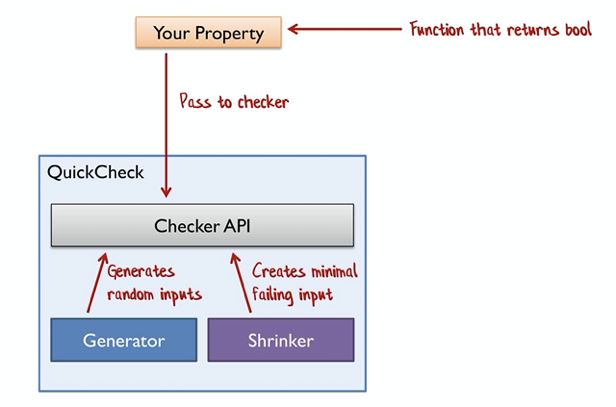
\includegraphics[width=1\textwidth]{images/schema.png}
                \caption{Schemat działania QuickCheck}
            \end{figure}    
        \end{columns}
    \end{frame}
    
    \begin{frame}{Funkcje QuickCheck}
    \begin{itemize}
        \item \textbf{Check.Quick} -- uruchamia szybki test, sprawdzając właściwość dla domyślnej liczby losowych przypadków (np. 100).
        \item \textbf{Check.Verbose} -- działa jak Check.Quick, ale wyświetla więcej szczegółowych informacji o danych testowych.
        \item \textbf{Generowanie danych wejściowych} -- FsCheck wspiera generowanie danych dla typów prostych (np. \texttt{int}, \texttt{float}, \texttt{string}) i bardziej złożonych struktur, takich jak listy czy rekordy.
    \end{itemize}
    \end{frame}
    
    \section{FsCheck}
    
    \begin{frame}[fragile]{Pisanie właściwości w FsCheck}
    FsCheck umożliwia definiowanie właściwości w formie funkcji logicznych. Właściwości opisują, jakie warunki zawsze muszą być spełnione przez funkcję.
    \begin{itemize}
        \item Odwrócenie listy dwukrotnie powinno zwrócić pierwotną listę.
    \end{itemize}
    \begin{lstlisting}[language=FSharp, xleftmargin=-10pt,xrightmargin=-10pt,numbers=none]
    let reverseProperty (xs: int list) =
        List.rev (List.rev xs) = xs

    Check.Quick reverseProperty
    \end{lstlisting}
    \end{frame}
    
    \begin{frame}{Generacja danych testowych}
    FsCheck pozwala na tworzenie własnych generatorów danych wybranego typu.
    \begin{itemize}
        \item Tworzenie generatora.
        \item Generowanie danych testowych dla różnych struktur.
        \item Wykorzystanie arbitrażu (Arb) do definiowania generatorów.
    \end{itemize}
    \end{frame}
    
    \begin{frame}[fragile]{Generatory}
    \begin{lstlisting}[language=FSharp, xleftmargin=-10pt,xrightmargin=-10pt,numbers=none,basicstyle=\ttfamily\small]
    let intGenerator = Arb.generate<int>
    Gen.sample 100 3 intGenerator  // [-37; 24; -62]
    type PositiveInt = PositiveInt of int  
    let positiveIntGen =
        Gen.suchThat ((<) 0) Arb.generate<int>
    Arb.register<PositiveInt>(positiveIntGen)     
    type Generators =
        static member PositiveInt() =
            Arb.fromGen positiveIntGen
    Arb.register<Generators>() // rejestracja generatora
    let intListGenerator = Arb.generate<int list>
    Gen.sample 5 10 intListGenerator 
    // [ []; []; [-4]; [0; 3; -1; 2]; [1]; [1]; []; [0; 1; -2]; [];]  
    let stringGenerator = Arb.generate<string>
    Gen.sample 10 3 stringGenerator // [""; "eiX$a^"; "U%0Ika&r"]     
    \end{lstlisting}
    \end{frame}
    
    \begin{frame}[fragile]{Przykład generatora dla złożonych struktur}
    \begin{lstlisting}[language=FSharp, xleftmargin=-10pt,xrightmargin=-10pt,numbers=none]
    type Point = {x:int; y:int; color: Color}
    let pointGenerator = Arb.generate<Point>
    Gen.sample 50 10 pointGenerator
    (*
    {x = -8; y = 12; color = Green -4;};
        {x = 28; y = -31; color = Green -6;};
        {x = 11; y = 27; color = Red;};
        {x = -2; y = -13; color = Red;};
        {x = 6; y = 12; color = Red;};
        // itd
    *)
    \end{lstlisting}
    \end{frame}
    
    \begin{frame}[fragile]{Shrinking}
    Proces redukcji danych wejściowych, który minimalizuje przypadki testowe prowadzące do błędu.
    \begin{itemize}
        \item Redukcja liczb do coraz mniejszych wartości.
        \item Redukcja ciągów znaków.
    \end{itemize}
    \begin{lstlisting}[language=FSharp, xleftmargin=-40pt,xrightmargin=-10pt,numbers=none]
        Arb.shrink "abcd" |> Seq.toList
        //["bcd"; "acd"; "abd"; "abc"; "abca"; "abcb"; "abcc"; "abad"]
    \end{lstlisting}
    \end{frame}
    
    \begin{frame}[fragile]{Shrinkowanie}
        \begin{lstlisting}[language=FSharp, xleftmargin=-10pt,xrightmargin=-10pt,numbers=none,basicstyle=\ttfamily\small]
    let isSmallerThan80 x = x < 80
    isSmallerThan80 100 // false, so start shrinking

    Arb.shrink 100 |> Seq.toList//  [0; 50; 75; 83; 94; 97; 99]
    isSmallerThan80 0 // true
    isSmallerThan80 50 // true
    isSmallerThan80 75 // true
    isSmallerThan80 83 // false, so shrink again

    Arb.shrink 83 |> Seq.toList//  [0; 44; 77; 79; 80; 81]
    isSmallerThan80 0 // true
    isSmallerThan80 44 // true
    isSmallerThan80 77 // true
    isSmallerThan80 79 // true
    isSmallerThan80 80 // false <- najmniejsza porazka
    // wynik: Falsifiable, after 10 tests (2 shrinks)
        \end{lstlisting}
    \end{frame}
    
    \begin{frame}[fragile]{Dostosowanie konfiguracji testów}
    \begin{lstlisting}[language=FSharp, xleftmargin=-10pt,xrightmargin=-10pt,numbers=none]
    let config = {
        Config.Quick with
            MaxTest = 1000
        }
        Check.One(config,isSmallerThan80 )
        // result: Ok, passed 1000 tests. (a nie powinno :)
        
        let config = {
        Config.Quick with
            MaxTest = 10000
        }
        Check.One(config,isSmallerThan80 )
        // result: Falsifiable, after 8660 tests (1 shrink):
        //         80
    \end{lstlisting}
    \end{frame}
    
    \begin{frame}[fragile]{Dodawanie warunków wstępnych}
    \begin{lstlisting}[language=FSharp, xleftmargin=-10pt,xrightmargin=-10pt,numbers=none]
    let preCondition x y =
        (x,y) <> (0,0)
        && (x,y) <> (2,2)

    let additionIsNotMultiplication_withPreCondition x y =
    preCondition x y ==> additionIsNotMultiplication x y
    // Ok, passed 100 tests.
    \end{lstlisting}
    \end{frame}
    
    \begin{frame}[fragile]{Testowanie wielu właściwości jednocześnie}
    \begin{lstlisting}[language=FSharp, xleftmargin=-10pt,xrightmargin=-10pt,numbers=none,basicstyle=\ttfamily\small]
    type AdditionSpecification =
        static member ``Commutative`` x y =
            commutativeProperty x y
        static member ``Associative`` x y z =
            associativeProperty x y z
        static member ``Left Identity`` x =
            leftIdentityProperty x
        static member ``Right Identity`` x =
            rightIdentityProperty x

    Check.QuickAll<AdditionSpecification>()
    --- Checking AdditionSpecification ---
    AdditionSpecification.Commutative-Ok, passed 100 tests.
    AdditionSpecification.Associative-Ok, passed 100 tests.
    AdditionSpecification.Left Identity-Ok, passed 100 tests.
    AdditionSpecification.Right Identity-Ok, passed 100 tests.
    \end{lstlisting}
    \end{frame}